\documentclass[border=4pt]{standalone}

\usepackage{amsmath}
\usepackage{tikz}
\usepackage{mathdots}
\usepackage{yhmath}
\usepackage{cancel}
\usepackage{color}
\usepackage{siunitx}
\usepackage{array}
\usepackage{multirow}
\usepackage{amssymb}
\usepackage{gensymb}
\usepackage{tabularx}
\usepackage{booktabs}
\usetikzlibrary{fadings}
\usetikzlibrary{patterns}
\usetikzlibrary{shadows.blur}
\usetikzlibrary{shapes}
 

\begin{document}



\tikzset{every picture/.style={line width=0.75pt}} %set default line width to 0.75pt        

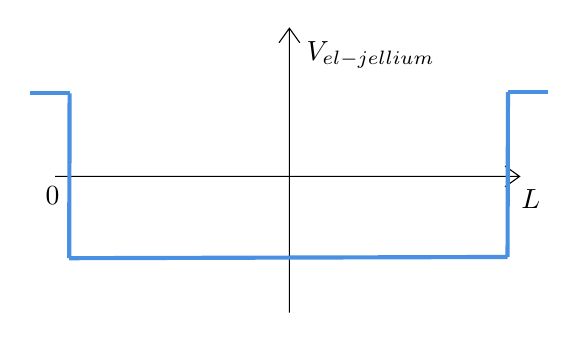
\begin{tikzpicture}[x=0.75pt,y=0.75pt,yscale=-1,xscale=1]
%uncomment if require: \path (0,300); %set diagram left start at 0, and has height of 300

%Shape: Axis 2D [id:dp025386996087595204] 
\draw  (38.8,107.4) -- (262.6,107.4)(151.69,36) -- (151.69,173) (255.6,102.4) -- (262.6,107.4) -- (255.6,112.4) (146.69,43) -- (151.69,36) -- (156.69,43)  ;

%Straight Lines [id:da8090444243940069] 
\draw [color={rgb, 255:red, 74; green, 144; blue, 226 }  ,draw opacity=1 ][line width=1.5]    (257,66.8) -- (256.8,146.2) ;
%Straight Lines [id:da8092416707167847] 
\draw [color={rgb, 255:red, 74; green, 144; blue, 226 }  ,draw opacity=1 ][line width=1.5]    (257,66.8) -- (276.2,66.8) ;
%Straight Lines [id:da8225543084708997] 
\draw [color={rgb, 255:red, 74; green, 144; blue, 226 }  ,draw opacity=1 ][line width=1.5]    (26.6,67.4) -- (45.8,67.4) ;
%Straight Lines [id:da3322579919993238] 
\draw [color={rgb, 255:red, 74; green, 144; blue, 226 }  ,draw opacity=1 ][line width=1.5]    (45.8,67.4) -- (45.6,146.8) ;
%Straight Lines [id:da12101716373692506] 
\draw [color={rgb, 255:red, 74; green, 144; blue, 226 }  ,draw opacity=1 ][line width=1.5]    (45.6,146.8) -- (256.8,146.2) ;

% Text Node
\draw (190.8,48.8) node    {$V_{el-jellium}$};
% Text Node
\draw (37.6,116.6) node    {$0$};
% Text Node
\draw (268,118.4) node    {$L$};


\end{tikzpicture}


\end{document}
